\chapter{\uppercase{Xen Hypervisor}}
Xen is an open-source hypervisor, that started as a project at University of Cambridge. It uses paravirtualization in conjunction with hardware assisted virtualization technologies to develop a VMM. Along with widespread adoption, it also boasts of native support from Linux kernel. 

\section{Xen Architecture}

Xen hypervisor follows a minimalist design policy with emphasis on security and efficiency. This is extremely important as the hypervisor hosts multiple Virtual Machines and any bugs may compromise the entire system. Virtual machines are hosted on custom environments called domains. Xen exposes very basic functionalities to these domains having similar UNIX counterparts as shown in Table~\ref{tab:unixcomp}. Guest OSes should contain relevant modifications to use these features. 

\begin{table}[H]
\centering
%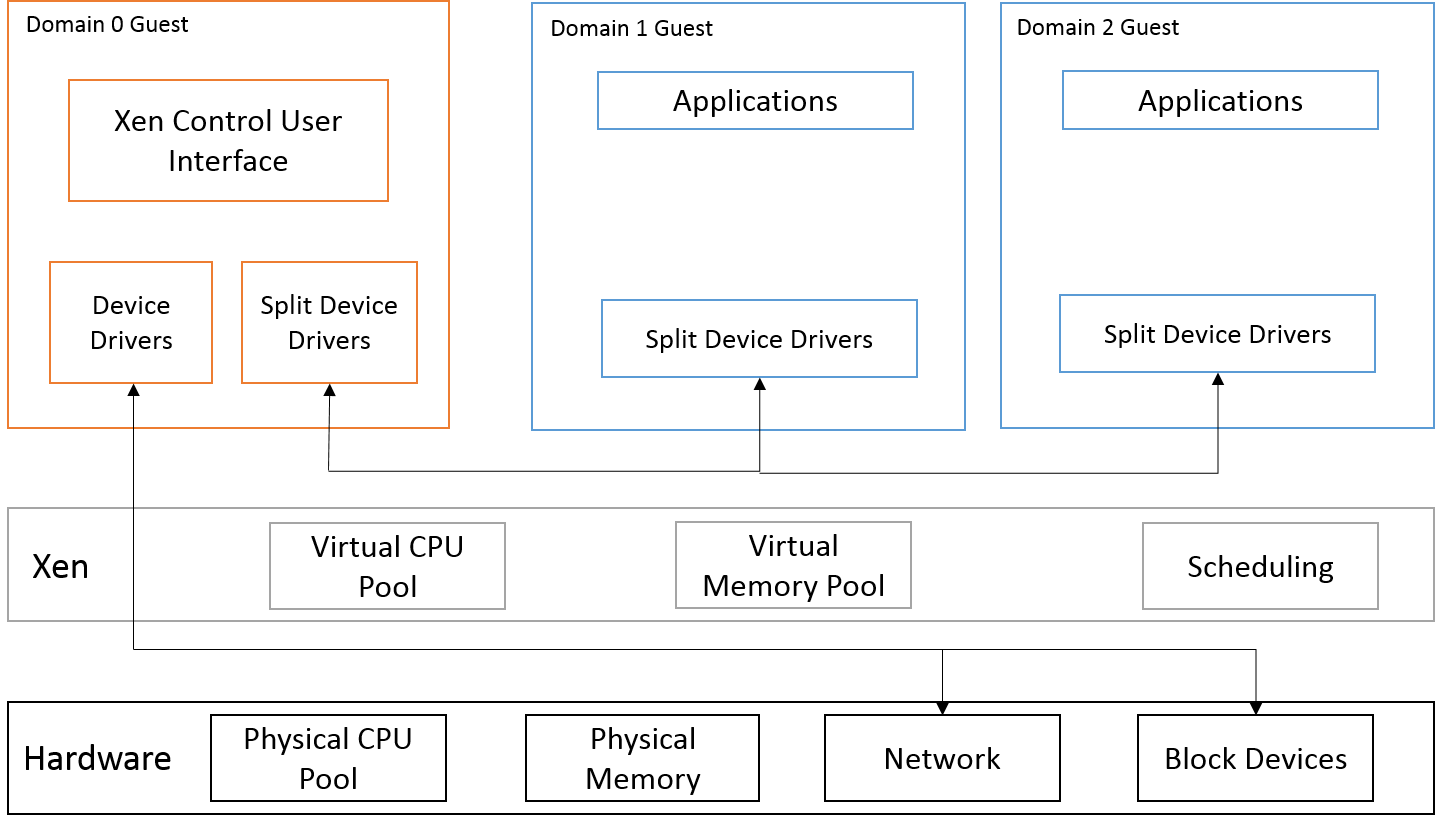
\includegraphics[scale=0.6]{figures/Xen_model.png}
\begin{tabular}{|c|c|}
    \hline
    UNIX & Xen \\
    \hline
    \hline
    System Calls & Hypercalls \\
    \hline
    Signals & Events \\
    \hline
    File system & Xenstore \\
    \hline
    POSIX shared memory & Grant tables  \\
    \hline
\end{tabular}
\caption[Comparison between Xen and Unix architecture]{Comparison between Xen and Unix architecture \cite{chisnall_book}}
\label{tab:unixcomp}
\end{table}

Initially Xen was designed undertaking paravirtualization on x86, i.e. Guest OS kernels were modified to be compatible with Xen. However, with the addition of Intel VT-x and AMD SVM extensions to the x86 architecture, it is possible to support pure virtualization. Guests on newer machines can run in two modes -- PV (Paravirtual) guest or HVM (Hardware Virtual Machine) Guest. In HVM mode, Xen can run guests without any source code modifications. On the other hand, running a paravirtualized guest kernel in HVM takes the hybrid approach where the guest may take advantage of hardware features (such as Nested Page Tables), in addition to the performance boosts provided by paravirtualization techniques (such as hypercalls). Guests can use the CPUID instruction to probe whether it is running directly on hardware, or on top of Xen.

The trap and emulate model, for hypervisors, is very expensive in terms of CPU cycles. Thus sensitive operations in a guest OS are typically replaced with hypercalls. This is quite similar to system calls in UNIX. Typically system calls use interrupt 80h (or SYSENTER instruction) to transfer control to the kernel in ring 0 with arguments either placed on the stack or in ISA registers. Hypercalls work in much the same way utilizing interrupt 82h instead in PV mode. However, in HVM mode, most interrupts are generally configured to be fed to the guest kernel instead of Xen. To enter the hypervisor at ring -1, a special instruction, VMCALL, is used instead.

These two separate methods are unified in newer Xen versions via calling an address at a certain offset in a special page mapped to the Guest OS's address space. The offset determines the specific hypercall command. In the above method, the hypercall issue procedure remains the same from the Guest OS kernel's perspective whether in PV mode or in HVM mode. The implementation specifics are hidden in the page mapped to the Guest VM.

In a Xen based system (Fig \ref{fig:xen_model}), memory and CPU resources are managed directly by the hypervisor, but I/O devices are generally controlled using a privileged domain (generally dom0). This domain runs at a higher privilege level where it is given direct access to many hardware resources. In addition to handling I/O operations, it also hosts the Xen User Interface used for administrative tasks. Thus, its security is of prime importance. Some of its responsibilities, such as hosting a device driver, may be delegated to domU guests (Guest domains) running at a higher privilege level. This feature is very useful in the case of a buggy device driver, as during any device driver related fault, only the specific domU needs to be restarted instead of the entire system. However, in the absence of IOMMU, DMA requests from this domain may potentially affect memory regions allocated to other VMs. 

\begin{figure}[H]
\centering
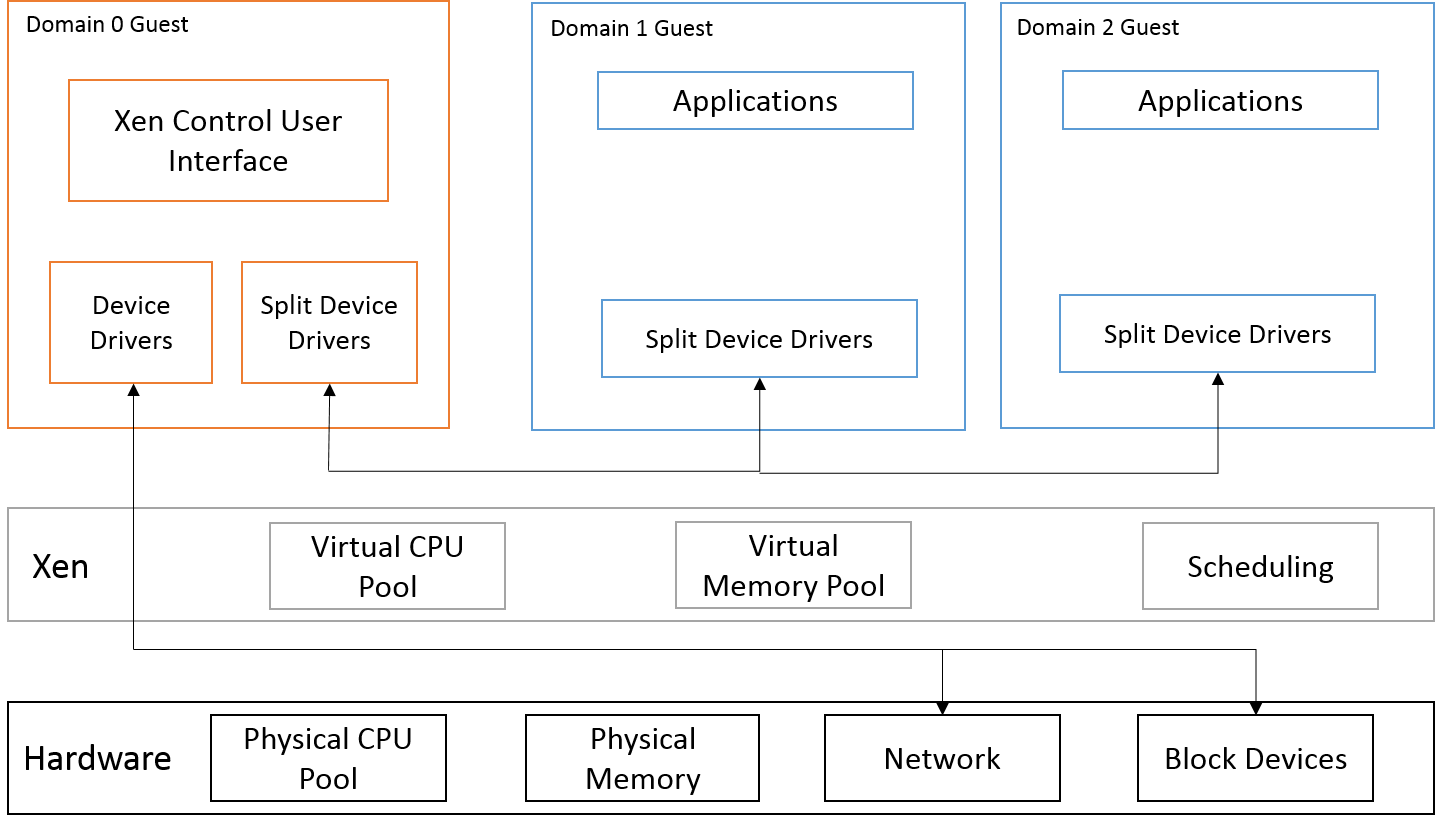
\includegraphics[scale=0.6]{figures/Xen_model.png}
\caption[Xen Architecture]{Xen Architecture \cite{chisnall_book}}
\label{fig:xen_model}
\end{figure}
Memory sharing in Xen is enabled via Grant tables. Memory is shared or transferred among domains at page granularity. This feature is quite useful in many situations such as networking among guests and implementing split device driver model.

One of the features of Xen which makes it very popular is its I/O interface. Xen escapes the need to both emulate devices and develop separate device drivers with a split device driver model. It is made up of the following.

1. Actual device driver.

2. Generic backend driver.

3. Generic frontend driver.

4. Ring buffer.

Typically, dom0 or a driver domain hosts the actual device drivers eliminating a notable amount of redundant developmental work. A generic frontend device driver is implemented in the guest domain at a much higher abstraction level which communicates with the backend device driver using ring buffers. The backend driver deconstructs the I/O requests from the front end driver and forwards it to the actual device driver. The requests are thus kept very simple avoiding device specific details. Ring buffers handle data movement across domains using shared memory utilities provided by Xen (Grant tables). A key advantage of this model is that a single split device driver can cover a whole class of devices.

Time keeping is another important aspect of an Operating System, especially for a scheduler. CPUs are shared amongst the running processes on a time sharing basis, and thus it is of utmost importance that the Operating System has accurate CPU clock information. Additionally, several user space applications also need wall clock time information, which can be calculated from system time. Usually the above is gathered using the CPU clock and network time information. However, in a virtual machine the CPU clock does not reflect the system time, because different Operating Systems share the same CPU. The hypervisor holds the responsibility to provide a virtual machine with system time corresponding to the actual time the VM occupies a CPU. In HVM domains, Xen receives support from the hardware extensions, while in PV domain the above is performed entirely in software. 

\section{Xen Control Interface}
The control interface of Xen contains a combination of user space, and kernel space code, through which hypercalls are issued. To host the interface, dom0 must comprise of a compliant kernel (Linux, NetBSD, Solaris, etc.) containing requisite modifications. The process stack, including and above the Xend daemon (Fig \ref{fig:xen_api}), run as user space applications while the rest run at a higher privilege level. 

\begin{figure}[H]
\centering
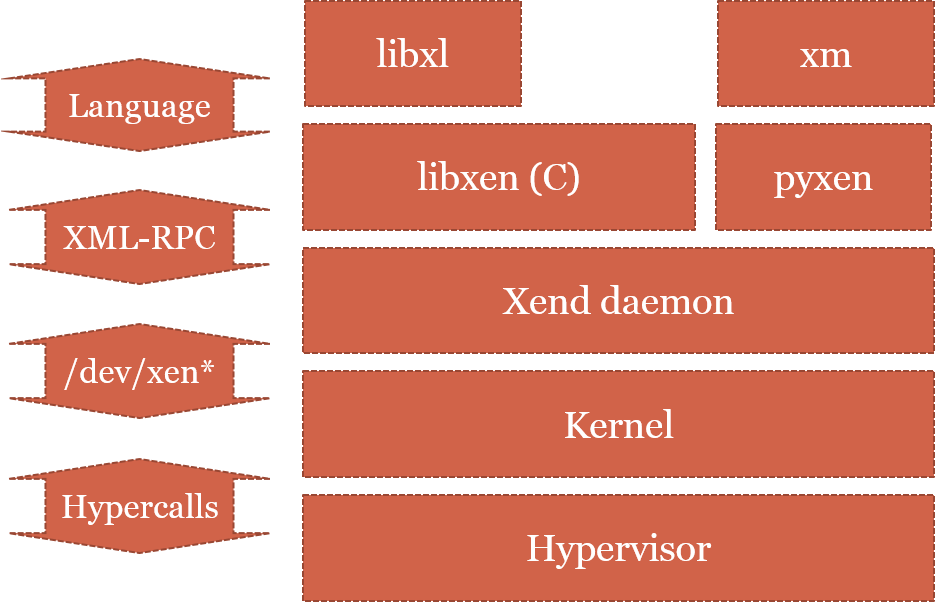
\includegraphics[scale=0.7]{figures/XEN_API.png}
\caption[Xen API]{Xen API \cite{chisnall_book}}
\label{fig:xen_api}
\end{figure}
Xen commands issued through any tool, are converted to XML-RPC messages to communicate with the Xend daemon. Xend daemon forwards the command to the kernel to issue hypercalls. In this chain of flow, the interface of Xend daemon is standardized through the definition of Xen API. This allows development and proliferation of user space management tools independent of changes lower in the stack. The complete Xen Control Interface structure is presented in Fig \ref{fig:xen_api}. Xen commands can be issued from a variety of user space tools such as xl, xm, libvirt, etc. Some tools (e.g. xm) written in python, have an additional overhead of a runtime python environment. In contrast, xl is relatively lightweight using libxen library, written in C, to generate XML-RPC messages.

The xend daemon runs in the user space, thus minimizing dependence on a specific kernel. On receiving messages, xend performs certain critical tasks such as access control and issues hypercalls to the hypervisor through the kernel.

Sample commands for xl toolchain are illustrated below:

\begin{itemize}
\item Create or start a virtual machine: xl create \textless config\_filename\textgreater

\item Shutdown a virtual machine: xl shutdown \textless domain\_id\textgreater
\end{itemize}


\section{Xen Memory Model}

Memory management is one of the core components of a hypervisor. With Xen core, the available memory is shared dynamically amongst the different virtual machines. It also allows for thin provisioning, i.e., projecting more memory than the available system RAM using ballooning techniques.

As a part of design philosophy, Xen does not swap pages out of memory itself. Individual guest OSes’ are the best judges to identify cold pages and thus this job is left over to them. Using the balloon driver, Xen is able to mount or release memory pressure in a VM. When the hypervisor wants to reclaim pages from a VM, it inflates the balloon driver in the virtual machine. The balloon driver requests more memory from the OS, which swaps cold pages out and releases memory to the balloon driver. The latter returns those freed up memory pages to the hypervisor so that it can be allocated to an appropriate VM. During runtime, as the memory requirement reduces, Xen deflates the balloon and releases memory back to the VM. The balloon driver monitors a target memory value, set in Xenstore to dynamically balance the actual memory allocated to the guest. This target memory value (set through domain0) is usually smaller than the guest physical address space and reflects the intended actual memory allocation for that domain. 
 

\subsection{x86\_64 Memory management}
This subsection focuses on the memory management details for x86\_64 machines. While extending the x86 ISA to 64 bits, AMD cleaned up memory segmentation controls, leaving a continuous flat address space with page level controls. In x86\_64, virtual memory is 64 bits wide, currently allowing only 48 bit sign extended addresses \cite{intel_manual}. A typical system looks similar to Fig \ref{fig:x86_memspace}, having 128TB + 128TB accessible regions. 

\begin{figure}[H]
\centering
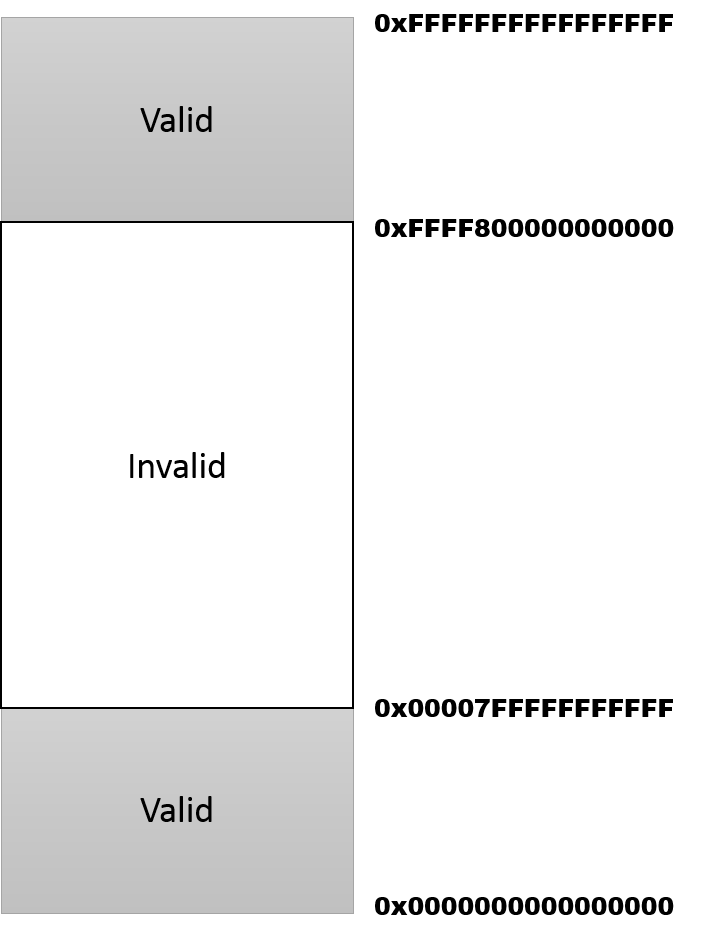
\includegraphics[scale=0.6]{figures/x86_64_VA_space.png}
\caption{x86\_64 Virtual Address Space}
\label{fig:x86_memspace}
\end{figure}

Typically for most Operating Systems, a virtual address space is generally divided into two parts

1. Kernel Space: This space is shared and common to all the applications. Kernel space also contains a direct mapping of the physical address space (usually with an offset).

2. Application Space: This space is specific to individual applications for application data and code.

For Linux on x86\_64 machines, the lower region goes to the application and the upper region is occupied by the kernel. Mapping the kernel into the individual application address spaces avoids the overhead of a context switch during a system call. Moreover, many system calls pass arguments via a pointer to a user space memory region, that is also accessible directly by the kernel, since the kernel is mapped onto the process address space. 

\begin{figure}[H]
\centering
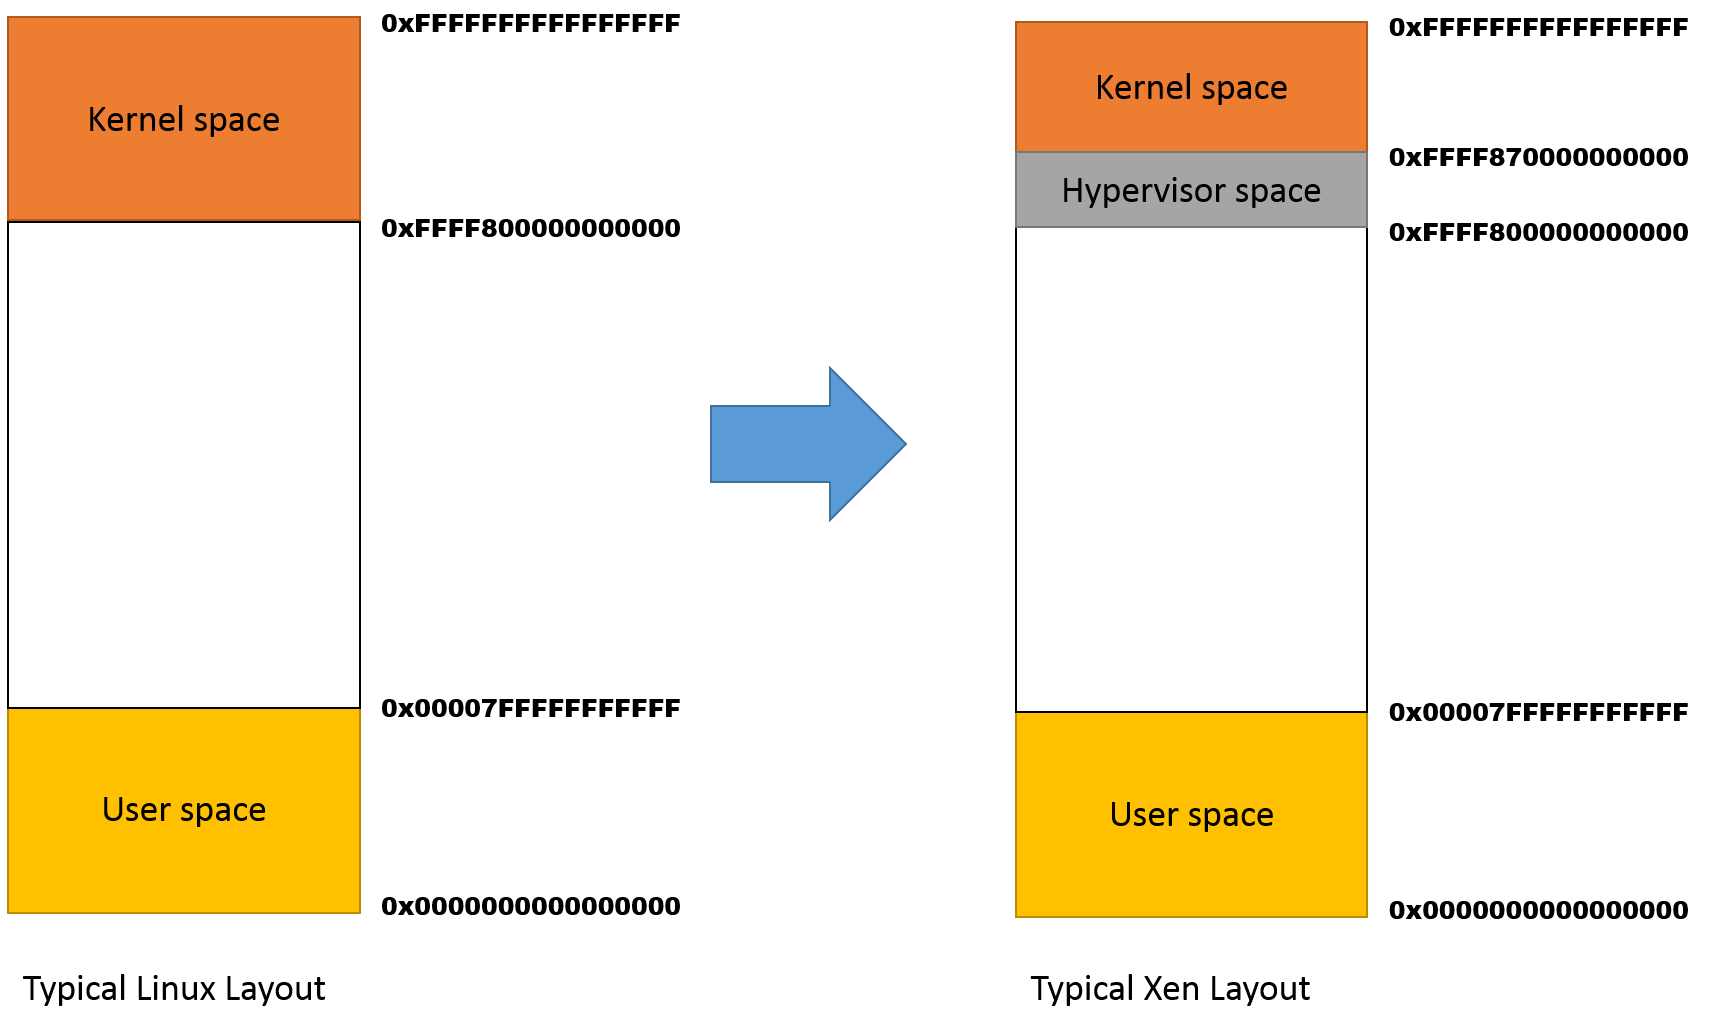
\includegraphics[scale=0.7]{figures/VA_layout_hypervisor.png}
\caption{Xen Virtual Address Layout Transformation}
\label{fig:xen_layout}
\end{figure}

A similar framework is setup in-between Xen hypervisor and the individual VMs (see Fig \ref{fig:xen_layout}). The hypervisor reserves a portion of the kernel address space for itself. This is done again to avoid context switches during hypercalls from a guest VM. This address space is again subdivided into different regions. 

%\begin{table}
%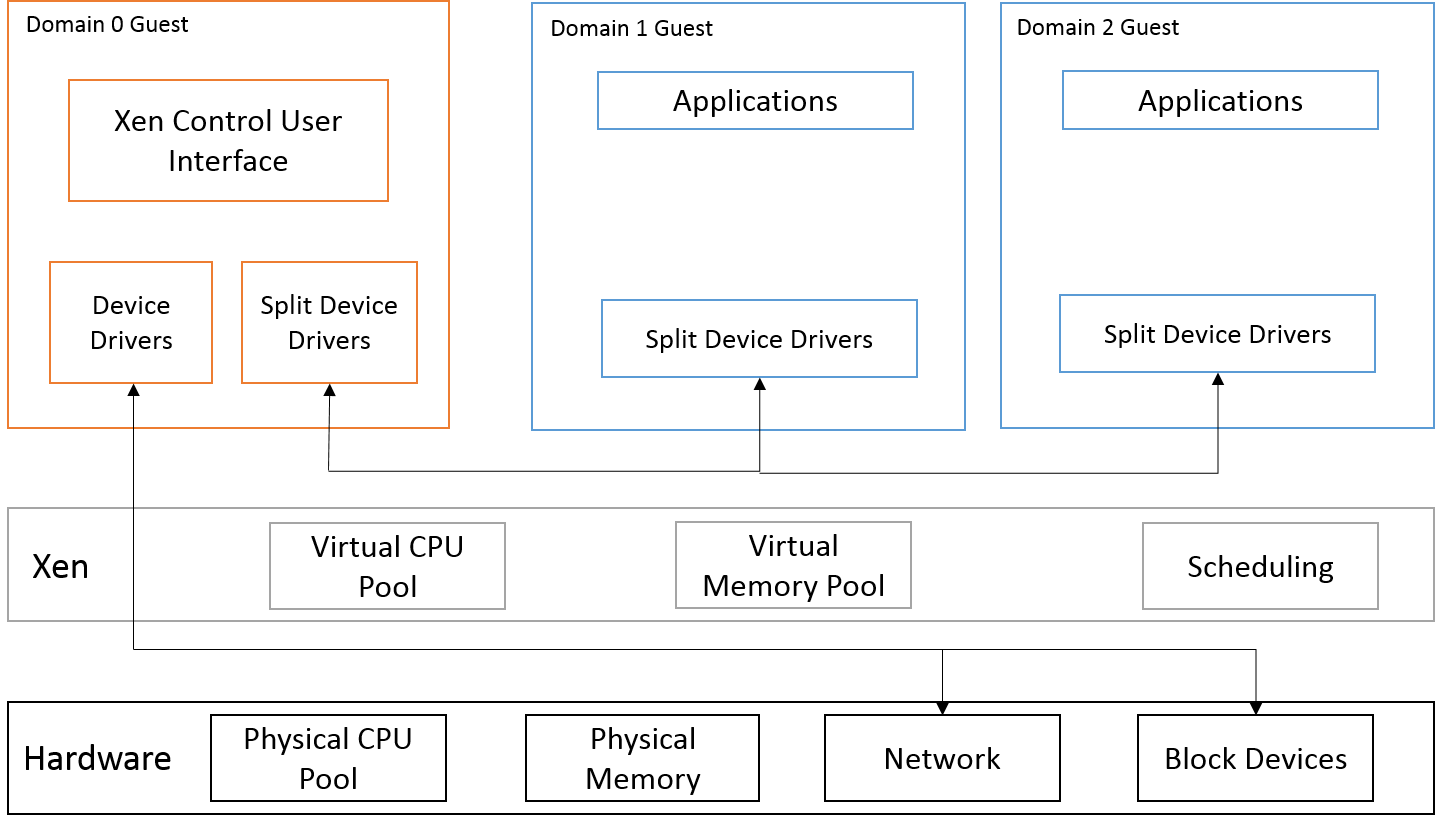
\includegraphics[scale=0.6]{figures/Xen_model.png}
\clearpage
\begin{longtable}{|m{2ex}|m{20ex}|m{18ex}|m{0.39\textwidth}|}
    \caption[Virtual Memory Regions]{Virtual Memory Regions \cite{xen_code} \label{tab:xen_address}}\\
    \hline
    & Start Address      & End Address        & Description \\
    \hline
    \hline
    \endfirsthead
    \hline
    \multicolumn{4}{|c|}{Continuation of Table \ref{tab:xen_address}}\\
    \hline
    \hline
    & Start Address      & End Address        & Description \\
    \hline
    \hline
    \endhead
    \hline
    \hline
    \multicolumn{4}{|c|}{\textit{Continued...}}\\
    \hline
    \endfoot
    \hline
    \hline
    \multicolumn{4}{|c|}{End of Table \ref{tab:xen_address}}\\
    \hline
    \endlastfoot
    1  & 0x0000000000000000  & 0x00007fffffffffff & [128TB, PML4:0-255] Guest-defined use \\
    \hline
    2  & 0x0000800000000000  & 0xffff7fffffffffff & [16EB] Inaccessible: Only 48-bit sign-extended VAs supported\\
    \hline
    3  & 0xffff800000000000  & 0xffff800000000000 & [256GB, PML4:256] Read-only machine-to-phys translation table (GUEST ACCESSIBLE) \\
    \hline
    4  & 0xffff804000000000  & 0xffff807fffffffff & [256GB, PML4:256] Reserved for future shared info with the guest OS (GUEST ACCESSIBLE) \\
    \hline
    5  & 0xffff808000000000  & 0xffff80ffffffffff & [512GB, PML4:257] ioremap for PCI mmconfig space \\
    \hline
    6  & 0xffff810000000000  & 0xffff817fffffffff & [512GB, PML4:258] Guest linear page table \\
    \hline
    7  & 0xffff818000000000  & 0xffff81ffffffffff & [512GB, PML4:259] Shadow linear page table \\
    \hline
    8  & 0xffff820000000000  & 0xffff827fffffffff & [512GB, PML4:260] Per-domain mappings (e.g., GDT, LDT) \\
    \hline
    9  & 0xffff828000000000  & 0xffff82bfffffffff & [256GB, PML4:261] Machine-to-phys translation table \\
    \hline
    10 & 0xffff82c000000000  & 0xffff82c3ffffffff & [16GB, PML4:261] ioremap()/fixmap area \\
    \hline
    11 & 0xffff82c400000000  & 0xffff82c43fffffff & [1GB, PML4:261] Compatibility machine-to-phys translation table \\
    \hline
    12 & 0xffff82c440000000  & 0xffff82c47fffffff & [1GB, PML4:261] High read-only compatibility machine-to-phys translation table \\
    \hline
    13 & 0xffff82c480000000  & 0xffff82c4bfffffff & [1GB, PML4:261] Xen text, static data, bss \\
    \hline
    14 & 0xffff82c4c0000000  & 0xffff82f5ffffffff & [197GB, PML4:261] Reserved for future use \\
    \hline
    15 & 0xffff82f600000000  & 0xffff82ffffffffff & [40GB, PML4:261] Page-frame information array \\
    \hline
    16 & 0xffff830000000000  & 0xffff87ffffffffff & [5TB, PML4:262-271] 1:1 direct mapping of all physical memory\\
    \hline
    17 & 0xffff880000000000  & 0xffffffffffffffff & [120TB, PML4:272-511] Guest-defined use.  \\
\end{longtable}

As seen in Table \ref{tab:xen_address}, different regions, serve individual purposes, while the complete machine memory is made directly accessible to Xen through region 16. 

\subsection{Hypercalls}

Several hypercalls are provided to facilitate common memory management operations in Xen. Although in a pure virtualization environment, it is not necessary, but hypercalls are included for performance gains.

Page table management is one of the most expensive operations in a paravirtualization approach. To prevent direct access to physical hardware, page tables of a domain are generally marked as read only by the hypervisor. Any attempted modifications by the guest VM would result in a trap to the VMM, which then emulates the required operation.

Xen provides hypercalls for the guest to make the above procedure easier. It also allows for multiple page table changes to be clubbed together, via the HYPERVISOR\_mmu\_update hypercall. However, these operations are not relevant to the case of an HVM guest. In x86 architecture, the VT-x (for Intel chips) and SVM (for AMD chips) extensions allow the guest direct access to its own page tables. This eliminates the scenario for traps altogether.

Thin provisioning is another important feature in a virtual machine. The balloon driver negotiates the actual memory occupied by a domain with the hypervisor. The popular commands used by it are XENMEM\_increase\_reservation, XENMEM\_decrease\_reservation and XENMEM\_populate\_physmap. The first two are used for runtime addition or removal of memory blocks behind the guest physical address space. While the third one is used for the initial mapping of the guest address space during domain creation, for large memory requests. These commands are executed through the HYPERVISOR\_memory\_op hypercall. Another important command associated with this hypercall is XENMEM\_memory\_map. It can replace the BIOS call to provide an E820 memory map to a paravirtualized guest. Though not necessary for domU guests, it is one of the available ways to determine the initial layout of guest physical address space. 


\chapter{\uppercase{Design and Implementation}}

Conception of the proposed system revolves around the design of an additional memory management unit in the hypervisor. Since NVM data has existence beyond the lifetime of a VM, the conventional MMU cannot be used. A new Non-volatile memory management unit is presented as a solution, for a popular hypervisor -- Xen.

In this chapter, several features of Xen are described relevant to the x86\_64 ISA with VT-x extensions and Intel Hub Architecture, followed by requisite modifications to incorporate the new MMU design. 

\section{Overview}
Boot procedure on x86 demands that the CPU should first transition from real mode to protected mode to access the entire address space. It should initialize the necessary page table data structure and segment registers to perform the switch while keeping interrupts masked during the transition process. After entering the protected mode the processor has a lot more flexibility, but typically loses access to BIOS calls. For the above mentioned reasons, bootstrapping on x86 is a quite complex and tricky procedure. Typically, initialization of a MMU is one of the first tasks for any kernel, and it involves a fair amount of bootstrapping code. It makes this undertaking all the more challenging and interesting.

Booting can also designate either the host machine startup or just starting a virtual machine. While the former is associated with the hypervisor taking stock of the hardware resources, the latter involves sharing the same with a VM in a secure manner. The major steps performed in a Xen based system from power on to starting a new domain is summarized in the flowchart presented in Fig \ref{fig:xen_flowchart} and Fig \ref{fig:dom_flowchart}. As evident from this figure this project can be broken down into two fundamental subdivisions.

1. Create an independent Memory Management Unit for the available Non-Volatile RAM.

2. Provide guest domains access to the NVRAM region, in a secure and protected manner. 


\begin{figure}[H]
\centering
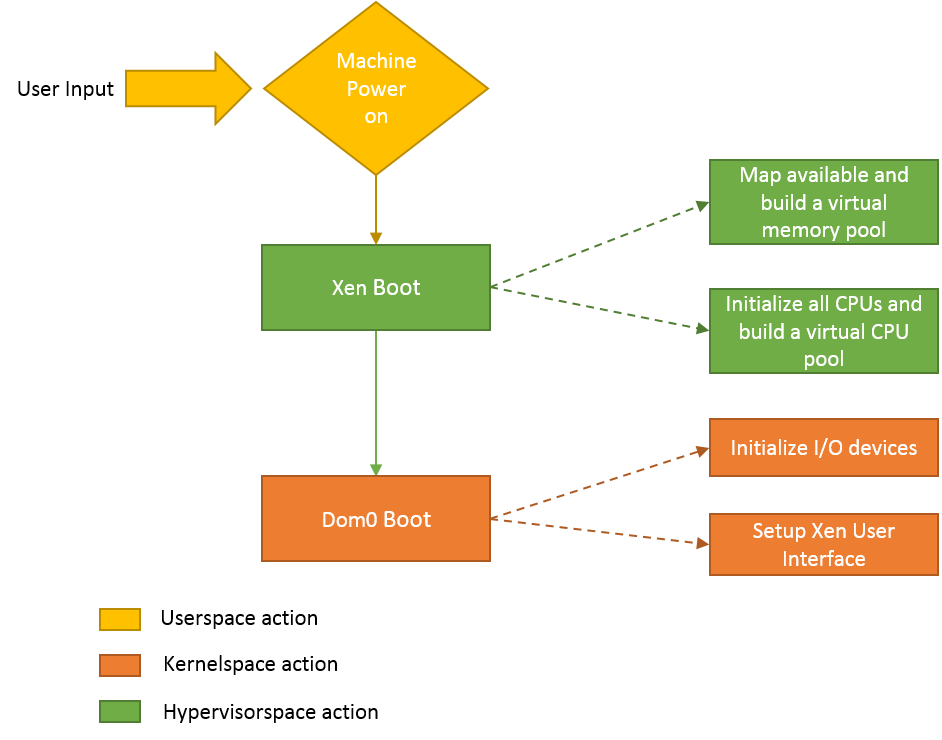
\includegraphics[scale=0.9]{figures/domain_creation1.png}
\caption{Domain Creation Flowchart : System Boot}
\label{fig:xen_flowchart}
\end{figure}

\begin{figure}[H]
\centering
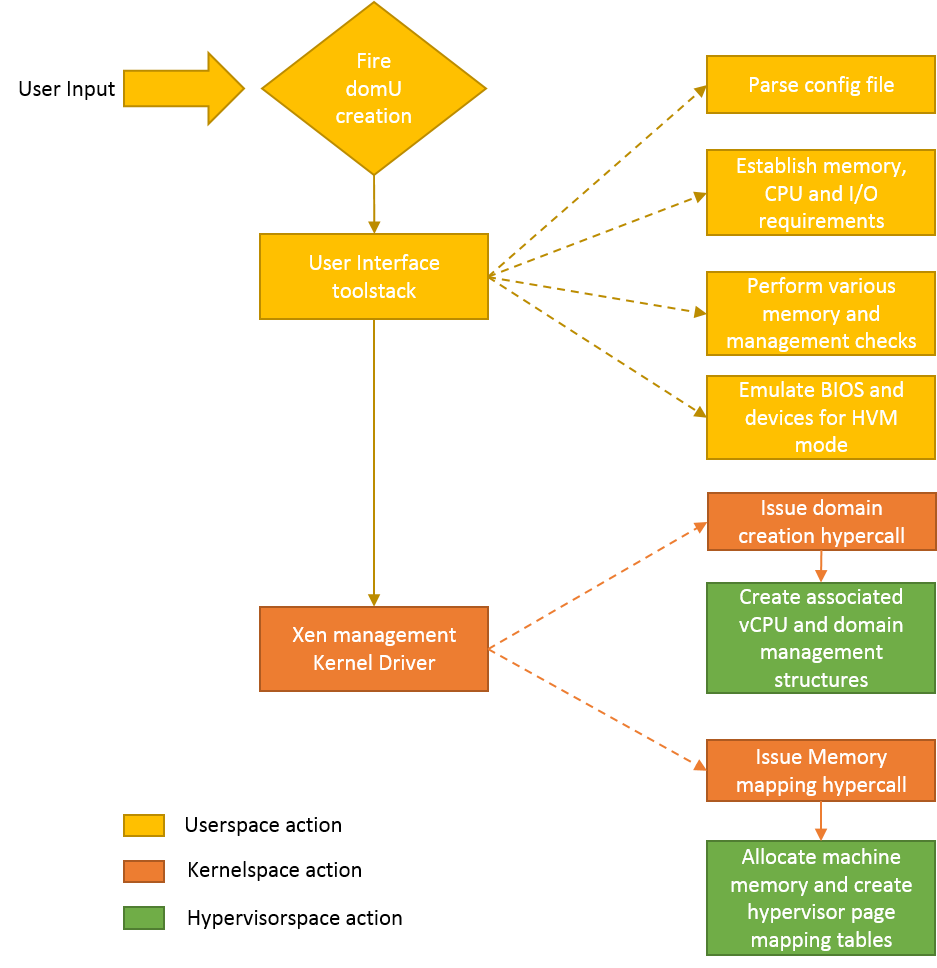
\includegraphics[scale=0.9]{figures/domain_creation2.png}
\caption{Domain Creation Flowchart : DomU Boot}
\label{fig:dom_flowchart}
\end{figure}
The first task requires modifications in the Xen kernel, with parts that deal with the boot process. Since the modifications are at the highest privilege level, it is very critical that the implementation be bug free, secure and efficient. Even minor bugs may cause the entire system to crash.

On the other hand, the second job deals more with user level code, specific to a toolchain. A notable part of domain creation focuses on emulation of firmware, performed mainly by various management tools. Only a small portion deals with issuing hypercalls for resource allocation. Therefore, in this section most of the implementation details reside in the Xen control interface with minor modifications to the hypercall structure. Due to standardization of Xen API, many tools have sprung up for VM management. This implementation picks up the xl toolchain, which is the default tool supported by Xen community.

A basic outline of the implementation is presented below, in Fig \ref{fig:xen_mod}, highlighting the modifications in red.

1. Recognize the presence of NVRAM from E820 memory map provided by BIOS.

2. Create a separate NVRAM pool to manage the resource independently.

3. Create separate interface to specify DomU RAM and NVRAM requirements.

4. Generate virtual E820 memory map reflecting the separate NVRAM pool.

5. Map the virtual NVRAM space in domUs to the physical Non-volatile memory present on the machine. 

\begin{figure}[H]
\centering
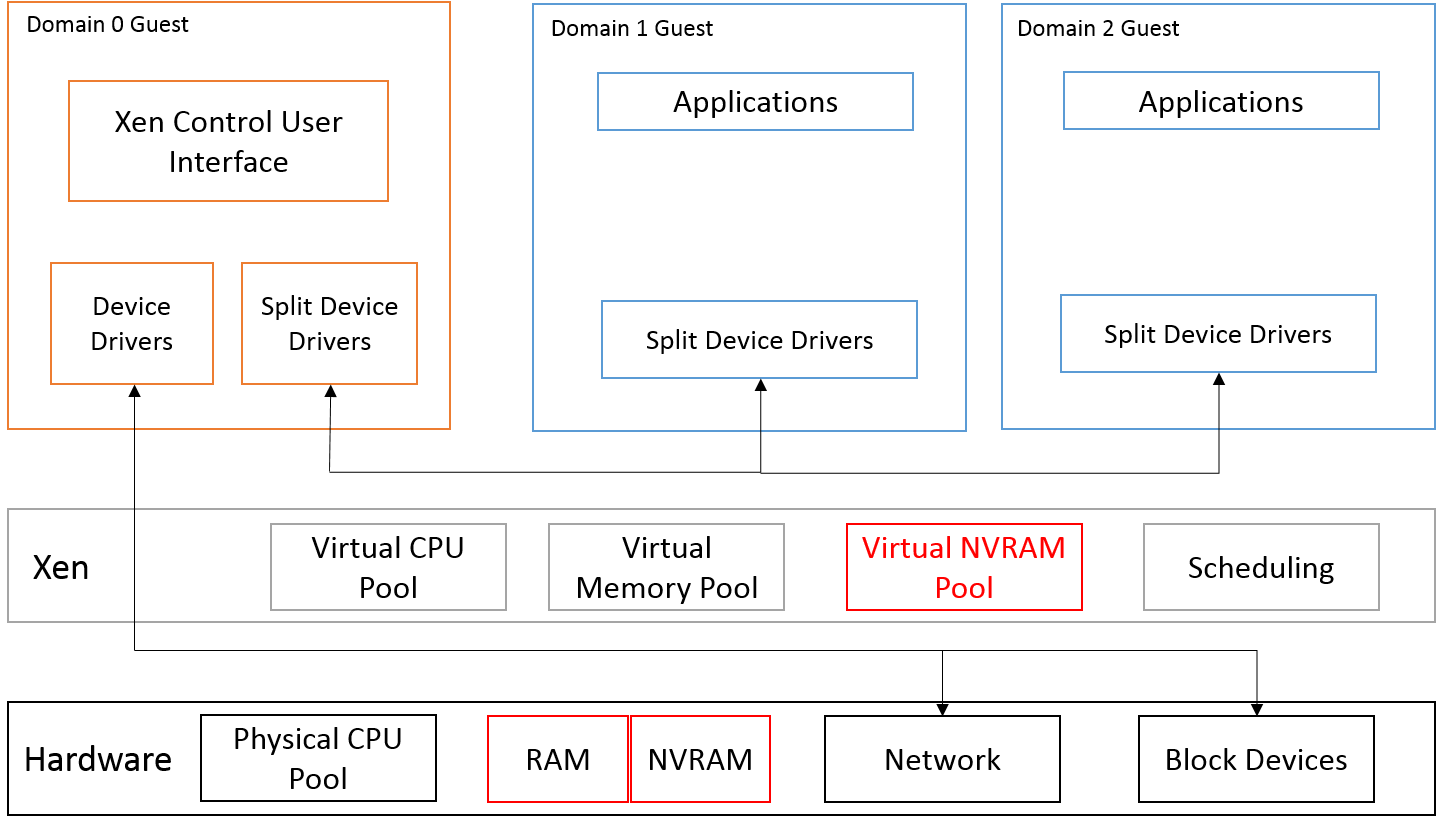
\includegraphics[scale=0.6]{figures/Xen_mod_model.png}
\caption{Modified Xen Architecture}
\label{fig:xen_mod}
\end{figure}

\section{Challenges}

There are several challenges faced during the design of the proposed system in Xen. The most notable being the absence of a modular design for system memory. Xen has been architected around volatile memory, and the notion of a homogeneous memory is integrated quite deep in the system design. This makes it all the more challenging to introduce another MMU. Moreover, a major portion of the initialization is done during the boot procedure, which is in itself quite a complex process for x86. Along with the above virtualization being a relatively new technology lacks sufficient documentation. Thus, even minor code changes turn into a grueling task. The combination of the above issues makes the implementation an arduous but exciting challenge. 


\section{Xen Boot Procedure}
On system start, Xen boots up first to take stock of the hardware present. It queries the BIOS for the E820 Memory map. Identifying the available memory regions, Xen builds preliminary page tables and switches the machine to protected mode. With paging enabled, the hypervisor can access the entire address space. It follows by building free page lists.

Each machine page is identified by a data structure called page\_info presented below \cite{xen_code}. This structure contains runtime administrative information about the machine pages such as status, domain identifier, special page status, order, etc. An array of these structures is initialized for all the machine pages as indicated in Fig \ref{fig:page_info_mapping}. This array of struct page\_info occupies the region 15 of Xen virtual address space identified in Table \ref{tab:xen_address}. Xen modifies this data structure to indicate any changes to the machine page. With predefined virtual address space regions for both the page\_info structures and the machine pages, a pointer to this structure can be used to calculate the virtual address of the corresponding page and vice versa. 

\smallskip
\begin{lstlisting}

 struct page_info
 {
     union {
         struct page_list_entry list;
         paddr_t up;
         uint64_t shr_handle;
     };
     /* Reference count and various PGC_xxx flags and fields. */
     unsigned long count_info;
     /* Context-dependent fields follow... */
     union {
         /* Page is in use: ((count_info & PGC_count_mask) != 0). */
         struct {
             /* Type reference count and various PGT_xxx flags and fields. */
             unsigned long type_info;
         } inuse;
         /* Page is in use as a shadow: count_info == 0. */
         struct {
             unsigned long type:5; /* What kind of shadow is this? */
             unsigned long pinned:1; /* Is the shadow pinned? */
             unsigned long head:1; /* Is this the first page of the shadow? */
             unsigned long count:25; /* Reference count */
         } sh;
         /* Page is on a free list: ((count_info & PGC_count_mask) == 0). */
         struct {
             /* Do TLBs need flushing for safety before next page use? */
             bool_t need_tlbflush;
         } free;
     } u;
     union {
         /* Page is in use, but not as a shadow. */
         struct {
             /* Owner of this page (zero if page is anonymous). */
             __pdx_t _domain;
         } inuse;
         /* Page is in use as a shadow. */
         struct {
             /* GMFN of guest page we're a shadow of. */
             __pdx_t back;
         } sh;
         /* Page is on a free list. */
         struct {
             /* Order-size of the free chunk this page is the head of. */
             unsigned int order;
         } free;
     } v;

     union {
         u32 tlbflush_timestamp;
         struct {
             u16 nr_validated_ptes;
             s8 partial_pte;
         };
         u32 shadow_flags;
         __pdx_t next_shadow;
     };
 }; 


\end{lstlisting}
 
\begin{figure}[H]
\centering
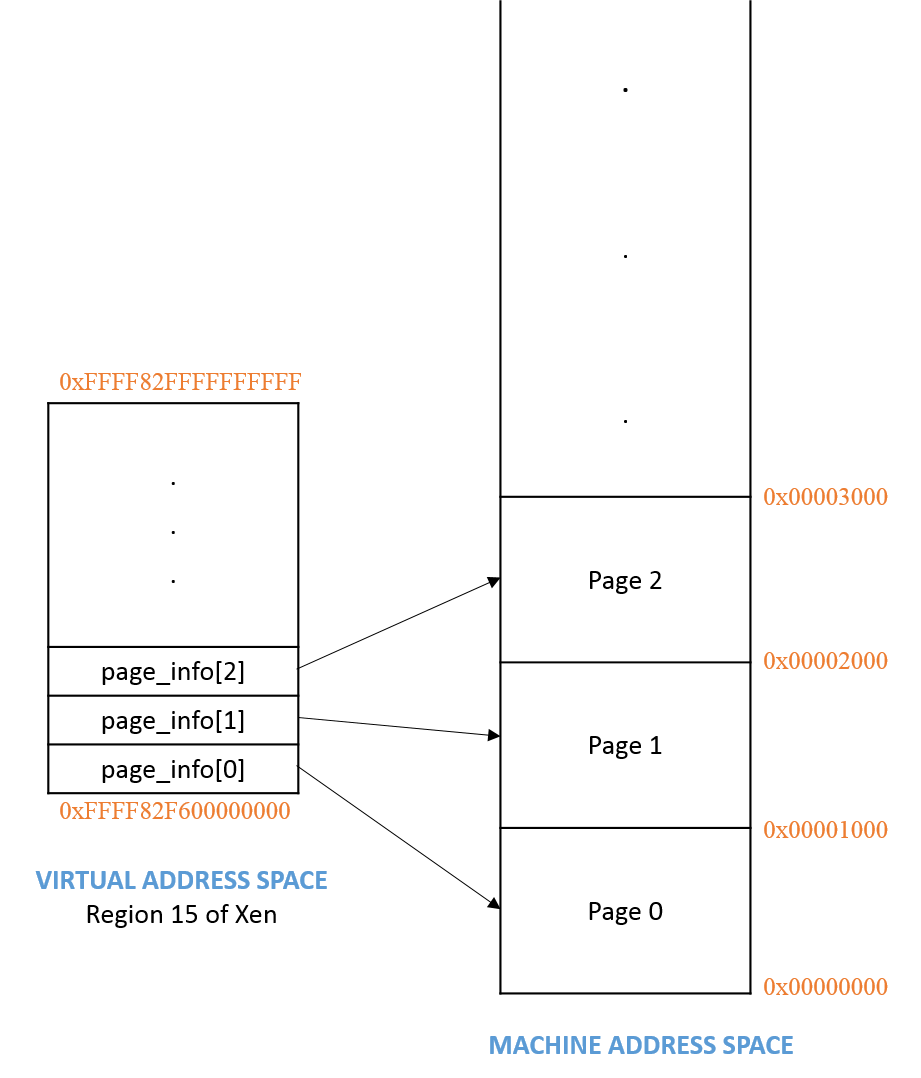
\includegraphics[scale=0.8]{figures/page_info.png}
\caption[Struct page\_info array to Machine Page mapping]{Struct page\_info array to Machine Page mapping \cite{xen_code}}
\label{fig:page_info_mapping}
\end{figure}

On system boot up, all the machine pages are free, without any domain affiliations. The Memory Management Unit builds a memory pool data structure \_heap[MEMZONE][ORDER] to manage and assimilate all the free pages. This \_heap data structure (Fig \ref{fig:heap_struct}) represents the free memory pool in Xen, arranging all the pages by MEMZONE and ORDER. Here MEMZONE divides the entire machine address space into different zones based on the position of the first non-zero bit in the address. This is necessary for special DMA memory requests for devices with fewer address bits. In each ZONE the pages are sorted by the order of the contiguous available pages up to a maximum of 1GB. 


\begin{figure}[H]
\centering
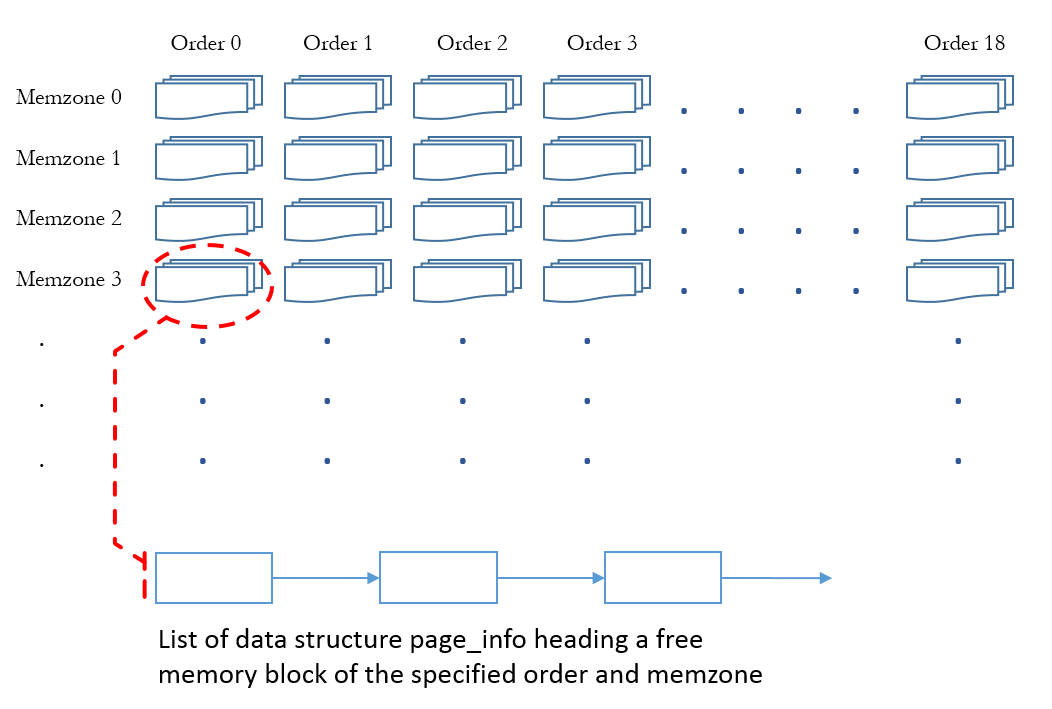
\includegraphics[scale=0.88]{figures/heap_data_structure.png}
\caption{Memory Pool -- \_heap data structure}
\label{fig:heap_struct}
\end{figure}

Each location in the 2-D array contains a list of the pages (actually their corresponding page\_info data structure) representing contiguous memory regions of the corresponding order and memzone. Memory requests are honored at page granularity by alloc\_heap\_pages and its wrapper functions, which extracts contiguous pages from the above \_heap data structure following a buddy system allocation. Pages returned by any domain are added to the memory pool using the free\_heap\_pages function call. This function coalesces any adjacent free regions, if available, and adds the memory pages back to the \_heap data structure. These pages are first scrubbed clean of all information before adding to the pool, protecting the security across domains. The pool is always aggregated to the highest order during these return requests.

Once the memory pool is ready, Domain 0 is given an appropriate amount of memory and the kernel image is copied. The hypervisor follows to build a CPU pool out of the available cores. It initializes VMCS and other associated data structures and hands control over to Domain0 Linux kernel. It is the responsibility of dom0 now to initialize all I/O devices using their appropriate drivers. 

\subsection{Design modifications}

 To enable sharing NVRAM across separate VMs, we have to first recognize it as a memory region. Currently the firmware (BIOS) marks that section with code 90. Due to lack of standardization, this code is subject to change and presently not recognized by Xen. Therefore, the hypervisor treats it as an unrecognized address space. Xen inhibits from either writing to or reading from these addresses.

The first task should be to recognize the memory region, and mark it as Non-Volatile RAM. A separate code word is added to the list of recognized E820 codes, to that effect. After identifying the region, a new NV memory pool is added in the form of an additional data structure \_nvm\_heap. This structure is quite similar to the \_heap data structure explained earlier except that it stores the pages of non-volatile memory. The E820 entries are examined one by one and the appropriate memory pools are populated, i.e. volatile RAM pool (identified by structure \_heap) is filled with RAM pages and non-volatile memory pool (identified by structure \_nvm\_heap) is filled with NVRAM pages.

Separate NVM allocator functions nvm\_alloc\_heap\_pages and nvm\_free\_heap\_pages are defined which operate on the \_nvm\_heap data structure. Similar to the volatile memory management function counterparts, these functions just manipulate the NV memory pool data structure and do not create any additional page table mappings. Since all pages are accessible via direct mapping and Xen does not perform swapping, page table modifications are not needed. The structure, page\_info, is also modified by adding a separate flag to differentiate between volatile and non-volatile pages.

With the above mentioned modifications in place, Xen is able to boot up, identify the available Non-volatile memory and allocate/de-allocate NVRAM pages on demand. A basic non-volatile memory management unit has been setup. It still requires an interface for domains to specify non-volatile memory requirements and request non-volatile memory through the NV MMU. The next section discusses a guest domain creation procedure, where modifications are added to utilize the above infrastructure. 

\section{Guest VM boot procedure}

Booting on bare metal x86 can be quite different from the virtual environment provided by Xen. An x86 CPU starts in 16 bit real mode, with BIOS providing basic essential functions such as hardware information, address space resolution and I/O device drivers. During the boot up procedure, the OS builds page tables and transitions the CPU to protected mode. At this point generally BIOS interrupt calls are unavailable so the OS device drivers are used for I/O. Most of the above functionalities are unavailable in a VM in Xen because the hypervisor boots up first transitioning the machine into protected mode. This poses a problem as the CPU state is totally different in a VM to what an Operating System is expecting.

A guest in Xen can boot in two available modes – PV and HVM. Both of them solve the above issue in separate ways. In PV mode, the OS kernel is modified to allow booting in protected mode. Due to unavailability of BIOS, boot time information is passed to the guest using shared memory pages. There are two types of shared memory pages.

1. Start info page: These pages are mapped to the guest’s address space by Xen. It provides necessary information such as total available memory (essentially the E820 memory map), number of virtual CPUs, console connection, and data structures regarding Xenstore. For boot purposes, Xen explicitly provides only a console device. Any other device must be mapped by the guest kernel using Xenstore services.

2. Shared info pages: A guest kernel needs to explicitly map these pages to its own address space for accessing dynamic runtime information about the virtual machine such as wall clock time, architectural information and event channels. This data is continually updated to reflect the status of the virtual machine.

Information provided through these channels helps in replacing BIOS functionality in PV guests.

HVM mode, on the other hand, is supposed to run unmodified OSes, thus it has to forgo some of the performance benefits of the PV mode and emulate certain devices. Emulation is not optimal because every abstract action is first converted to device specific commands by the guest OS device driver, and these commands are intercepted by Xen. The device emulator reconverts these device specific commands back to the abstract actions that are forwarded to the actual device driver for completion. The Xen split device driver model in PV guests generally runs at a higher level of abstraction avoiding most of the redundant work observed in emulation.

BIOS is emulated by borrowing code from Bochs emulator. It forms the front end in a split device driver model, with the back end handled by code borrowed from QEMU, which is used to emulate devices in HVM mode. Xen starts a domain from the BIOS start point in the virtual 8086 mode present in x86. This mode is actually intended for running legacy application in real mode, alongside protected mode applications. Since it was designed for userspace code, the boot code of an OS (containing a good amount of sensitive instructions) result in numerous traps which have to be handled individually by Xen.

In a hybrid approach, Paravirtualized guests can take the benefit of paravirtualization techniques as well as hardware accelerators while running in HVM mode. The guest can specify a location in its ELF header where the hypercall page can be loaded. It can also execute the CPUID instruction to determine whether it is running on top of Xen or bare metal hardware. If running on Xen, the guest may choose to switch over to Xen specific device drivers, and also map the hypercall page during runtime. However, all these functions are typically performed after the kernel boots up, thus BIOS and QEMU emulator are generally needed during boot-up.

Starting a domain begins with defining a configuration file that includes the disk storage, memory, vCPU and other parameters. The command xl create <filename> performs certain administrative tasks in the userspace domain and then fires up the domain. Initially, the xl tool parses the configuration file to identify resource requirements, most important of them being memory. If sufficient memory is not available, then an attempt is made to free up memory by communicating to Xen the additional memory requirement via Xenstore. This would typically result in Xen inflating the balloon drivers. In the event of still not meeting the memory requirement, the xl tool aborts the domain creation process with an error.

On the other hand, if the memory requirements are met, the tool issues a hypercall (via xend) to build necessary data structures (VMCS and internal Xen data structures) for domain management. The management tool also creates a guest physical address space and sends a hypercall for appropriate memory allocation and page-table mappings. The hypervisor, on receiving this hypercall, allocates pages via the associated functions mentioned in the previous section. It also builds up the hypervisor page tables to map the guest physical pages to actual machine pages. If all is successful then a virtual E820 memory map is created, and the new VM is booted with emulated firmware using code borrowed from Bochs and QEMU.

\subsection{Design modification}
The overall objective of this section is to create an interface for configuration and allocation of Non-volatile memory. Current work focuses on extending this functionality only for HVM guests. Here, implementation details lie in three areas – xl management tool, Bochs emulator, and hypercall structure.

First and foremost, a parameter is added to the configuration file facilitating the specification of the non-volatile memory requirement in Megabytes. This parameter is read by the tool chain, which then creates additional guest physical address space for NVRAM. Actual memory allocation is performed at this point using hypercalls to notify the hypervisor of the guest physical page numbers with emphasis on allocation of contiguous memory blocks to minimize TLB entries. The x86\_64 architecture provides page mapping in the sizes of 1GB, 2MB and 4KB. The allocator moves in descending order for memory requests to satisfy the requirement. A flag is added to the hypercall argument to differentiate between volatile and non-volatile memory requests. If the flag is set, the hypervisor pulls pages out of the NVRAM pool, else it uses the RAM pool for the purpose.

The above procedure completes one of the most critical portions of domain creation. Allocations of both volatile and non-volatile memory are complete and Xen is left with the task of firmware emulation. The toolchain creates virtual E820 table mappings, with an added region to indicate NVRAM with code 90. This completes the boot procedure and the virtual machine is equipped with non-volatile memory. When the VM is turned off, the hypervisor reclaims both RAM and NVRAM pages and adds them to their respective memory pools. 
